\documentclass{ximera}

\author{Anna Davis \and Paul Zachlin} \title{Matrix of a Linear Transformation with Respect to Arbitrary Bases} \license{CC-BY 4.0}

\renewcommand{\vec}[1]{{\bf #1}}
\newcommand{\RR}{\mathbb{R}}
\newcommand{\dfn}{\textit}
\newcommand{\dotp}{\cdot}


\newtheorem{general}{Generalization}
\newtheorem{initprob}{Exploration Problem}
\usepackage{tikz-cd}
\pgfplotsset{compat=1.14}



\begin{document}
\begin{abstract}
  We find the matrix of a linear transformation with respect to arbitrary bases, and find the matrix of an inverse linear transformation.
\end{abstract}
\maketitle

\section*{Examples of Matrices of Linear Transformations with Respect to  Arbitrary Bases}

\begin{initprob}\label{init:matlintransgeneral}
Let
$$\vec{v}_1=\begin{bmatrix}1\\2\\0\end{bmatrix}\quad\text{and}\quad\vec{v}_2=\begin{bmatrix}0\\1\\1\end{bmatrix}$$
$$\vec{w}_1=\begin{bmatrix}1\\0\\1\end{bmatrix}\quad\text{and}\quad\vec{w}_2=\begin{bmatrix}1\\0\\0\end{bmatrix}$$

In Example \ref{ex:subtosub1} of LTR-M-0025 we defined $V$ and $W$ as follows:

$$V=\text{span}(\vec{v}_1, \vec{v}_2)\quad\text{and}\quad W=\text{span}(\vec{w}_1, \vec{w}_2)$$

We chose
$$\mathcal{B}=\{\vec{v}_1, \vec{v}_2\}\quad\text{and}\quad\mathcal{C}=\{\vec{w}_1, \vec{w}_2\}$$
as bases of $V$ and $W$, respectively.

We also defined a linear transformation $T:V\rightarrow W$ by 
$$T(\vec{v}_1)=2\vec{w}_1-3\vec{w}_2\quad\text{and} \quad T(\vec{v}_2)=-\vec{w}_1+4\vec{w}_2$$

Our goal now is to find a matrix associated with this transformation.  

Why is it that we cannot find the standard matrix of $T$?\begin{hint}{Here the domain is a two-dimensional subspace of $\RR^3$, and such a subspace need not contain the standard basis vectors.}\end{hint} 

Recall that a transformation is completely determined by its action on a basis.  So, what our matrix needs to capture is this:
$$1\vec{v}_1+0\vec{v}_2\mapsto 2\vec{w}_1-3\vec{w}_2$$
$$0\vec{v}_1+1\vec{v}_2\mapsto -1\vec{w}_1+4\vec{w}_2$$
Because the bases vectors $\vec{v}_1$, $\vec{v}_2$, $\vec{w}_1$ and $\vec{w}_2$ are permanent fixtures in this set-up what we are really looking for is to capture what happens to the coefficients of $\vec{v}_1$, $\vec{v}_2$, $\vec{w}_1$ and $\vec{w}_2$.   Diagrammatically, we have:
$$\begin{bmatrix}1\\0\end{bmatrix}\mapsto\begin{bmatrix}2\\-3\end{bmatrix}$$
$$\begin{bmatrix}0\\1\end{bmatrix}\mapsto\begin{bmatrix}-1\\4\end{bmatrix}$$
Vectors $\begin{bmatrix}1\\0\end{bmatrix}$ and $\begin{bmatrix}0\\1\end{bmatrix}$ are said to be \dfn{coordinate vectors} of $\vec{v}_1$ and $\vec{v}_2$ with respect to $\mathcal{B}$, while $\begin{bmatrix}2\\-3\end{bmatrix}$ and $\begin{bmatrix}-1\\4\end{bmatrix}$ are the \dfn{coordinate vectors} of the images of $\vec{v}_1$ and $\vec{v}_2$ with respect to  $\mathcal{C}$. For now, we will refer to this mapping as a ``mapping of coordinate vectors".  But this mapping is induced by 
$$A=\begin{bmatrix}2&-1\\-3&4\end{bmatrix}$$
Let's take a look at what this matrix can do for us.

Recall that in Example \ref{ex:subtosub1} of LTR-M-0025 we found that the image of $\vec{v}=2\vec{v}_1+\vec{v}_2$ is $$T(\vec{v})=T(2\vec{v}_1+\vec{v}_2)=3\vec{w}_1-2\vec{w}_2$$
Utilizing our ``mapping of coordinate vectors" notation, we can express this as 
$$\begin{bmatrix}2\\1\end{bmatrix}\mapsto\begin{bmatrix}3\\-2\end{bmatrix}$$
Note that this result can be obtained by finding the product $A\begin{bmatrix}2\\1\end{bmatrix}$.
$$\begin{bmatrix}2&-1\\-3&4\end{bmatrix}\begin{bmatrix}2\\1\end{bmatrix}=\begin{bmatrix}3\\-2\end{bmatrix}$$

Given any vector $\vec{u}=a\vec{v}_1+b\vec{v}_2$ of $V$, we can find $T(\vec{u})$ as follows:
$$\begin{bmatrix}2&-1\\-3&4\end{bmatrix}\begin{bmatrix}a\\b\end{bmatrix}=\begin{bmatrix}2a-b\\-3a+4b\end{bmatrix}$$

This gives us
$$T(\vec{u})=T(a\vec{v}_1+b\vec{v}_2)=(2a-b)\vec{w}_1+(-3a+4b)\vec{w}_2$$

\end{initprob}

Matrix $A$ of Exploration Problem \ref{init:matlintransgeneral} is called the \dfn{matrix of linear transformation $T$ with respect to $\mathcal{B}$ and $\mathcal{C}$}.

\begin{example}\label{ex:transmatrix1}
Let $V$ and $W$ be vector spaces with bases $\mathcal{B}=\{\vec{v}_1, \vec{v}_2, \vec{v}_3\}$ and $\mathcal{C}=\{\vec{w}_1, \vec{w}_2\}$, respectively.  Define a linear transformation $T:V\rightarrow W$ by $$T(\vec{v}_1)=2\vec{w}_1-\vec{w}_2,\quad T(\vec{v}_2)=-\vec{w}_1,\quad T(\vec{v}_3)=\vec{w}_1+3\vec{w}_2$$
Find the matrix of $T$ with respect to $\mathcal{B}$ and $\mathcal{C}$, and use it to find $T(2\vec{v}_1-\vec{v}_2+3\vec{v}_3)$.  Verify your answer by computing $T(2\vec{v}_1-\vec{v}_2+3\vec{v}_3)$ directly.

\begin{explanation}
We will start by representing the action of $T$ on elements of $\mathcal{B}$ diagrammatically
$$1\vec{v}_1+0\vec{v}_2+0\vec{v}_3\mapsto 2\vec{w}_1+(-1)\vec{w}_2$$
$$0\vec{v}_1+1\vec{v}_2+0\vec{v}_3\mapsto (-1)\vec{w}_1+0\vec{w}_2$$
$$0\vec{v}_1+0\vec{v}_2+1\vec{v}_3\mapsto 1\vec{w}_1+3\vec{w}_2$$
This gives us the following ``mapping of coordinate vectors"
$$\begin{bmatrix}1\\0\\0\end{bmatrix}\mapsto \begin{bmatrix}2\\-1\end{bmatrix}$$
$$\begin{bmatrix}0\\1\\0\end{bmatrix}\mapsto \begin{bmatrix}-1\\0\end{bmatrix}$$
$$\begin{bmatrix}0\\0\\1\end{bmatrix}\mapsto \begin{bmatrix}1\\3\end{bmatrix}$$
The matrix of $T$ with respect to $\mathcal{B}$ and $\mathcal{C}$ is then given by
$$A=\begin{bmatrix}2&-1&1\\-1&0&3\end{bmatrix}$$
Applying this matrix to the coordinate vector of $2\vec{v}_1-\vec{v}_2+3\vec{v}_3$ we get
$$\begin{bmatrix}2&-1&1\\-1&0&3\end{bmatrix}\begin{bmatrix}2\\-1\\3\end{bmatrix}=\begin{bmatrix}8\\7\end{bmatrix}$$

This means that $T(2\vec{v}_1-\vec{v}_2+3\vec{v}_3)=8\vec{w}_1+7\vec{w}_2$.
We can verify this by direct computation as follows:
\begin{align*}
T(2\vec{v}_1-\vec{v}_2+3\vec{v}_3)&=2T(\vec{v}_1)-T(\vec{v}_2)+3T(\vec{v}_3)\\&=2(2\vec{w}_1-\vec{w}_2)-(-\vec{w}_1)+3(\vec{w}_1+3\vec{w}_2)\\&=8\vec{w}_1+7\vec{w}_2
\end{align*}
\end{explanation}

\end{example}

The following example shows that not only do the basis elements matter, but also their order.
\begin{example}\label{ex:transmatrix2}
Let $\mathcal{B}=\left\{\begin{bmatrix}0\\1\end{bmatrix},\begin{bmatrix}1\\0\end{bmatrix}\right\}$ be a basis for $\RR^2$ and let $\mathcal{C}=\left\{\begin{bmatrix}0\\0\\1\end{bmatrix},\begin{bmatrix}0\\1\\0\end{bmatrix}, \begin{bmatrix}1\\0\\0\end{bmatrix}\right\}$ be a basis for $\RR^3$.  Define a linear transformation $T:\RR^2\rightarrow \RR^3$ by 
$$T\left(\begin{bmatrix}0\\1\end{bmatrix}\right)=\begin{bmatrix}2\\0\\1\end{bmatrix}\quad\text{and}\quad T\left(\begin{bmatrix}1\\0\end{bmatrix}\right)=\begin{bmatrix}-1\\3\\4\end{bmatrix}$$
Find the matrix of $T$ with respect to $\mathcal{B}$ and $\mathcal{C}$.

\begin{explanation}
For simplicity, we will label the elements of $\mathcal{B}$
$$\vec{v}_1=\begin{bmatrix}0\\1\end{bmatrix},\quad\vec{v}_2=\begin{bmatrix}1\\0\end{bmatrix}$$
and elements of $\mathcal{C}$
$$\vec{w}_1=\begin{bmatrix}0\\0\\1\end{bmatrix},\quad\vec{w}_2=\begin{bmatrix}0\\1\\0\end{bmatrix},\quad\vec{w}_3=\begin{bmatrix}1\\0\\0\end{bmatrix}$$
Note the order of these vectors.  The order is very important!

Observe that $$T(\vec{v}_1)=\vec{w}_1+2\vec{w}_3,\quad T(\vec{v}_2)=4\vec{w}_1+3\vec{w}_2-\vec{w}_3$$

This gives us
$$1\vec{v}_1+0\vec{v}_2\mapsto 1\vec{w}_1+0\vec{w}_2+2\vec{w}_3$$
$$0\vec{v}_1+1\vec{v}_2\mapsto 4\vec{w}_1+3\vec{w}_2+(-1)\vec{w}_3$$

So, the ``mapping of coordinate vectors" looks like this

$$\begin{bmatrix}1\\0\end{bmatrix}\mapsto\begin{bmatrix}1\\0\\2\end{bmatrix}$$
$$\begin{bmatrix}0\\1\end{bmatrix}\mapsto\begin{bmatrix}4\\3\\-1\end{bmatrix}$$
The matrix of $T$ with respect to $\mathcal{B}$ and $\mathcal{C}$ is 
$$A=\begin{bmatrix}1&4\\0&3\\-1&2\end{bmatrix}$$

Compare this to the matrix of $T$ with respect to the standard basis (in standard order!).
\end{explanation}
\end{example}

\section{The Matrix of a Linear Transformation}
In this section we will formalize the process for finding the matrix of a linear transformation with respect to arbitrary bases that we established through earlier examples.

Let $V$ and $W$ be vector spaces with bases $\mathcal{B}=\{\vec{v}_1, \vec{v}_2,\ldots ,\vec{v}_n\}$ and $\mathcal{C}=\{\vec{w}_1, \vec{w}_2,\ldots ,\vec{w}_m\}$, respectively.   Suppose $T:V\rightarrow W$ is a linear transformation.  Our goal is to represent this transformation as a matrix transformation.

Observe that $\text{dim}(V)=n=\text{dim}(\RR^n)$ and $\text{dim}(W)=m=\text{dim}(\RR^m)$. Define a linear transformation $R:V\rightarrow \RR^n$ by $R(\vec{v}_i)=\vec{e}_i$ for $1\leq i\leq n$.  In Practice Problem \ref{prob:coordinatemappingisanisom} you will be asked to show that $R$ is one-to-one and onto.  This means that $R$ is an isomorphism.  (Compare this to Exploration Problem \ref{init:coordmapping} of LTR-M-0060)

Suppose $\vec{v}$ is an element of $V$, then $\vec{v}=a_1\vec{v}_1+a_2\vec{v}_2+\ldots +a_n\vec{v}_n$.  The image of $\vec{v}$ is given by
\begin{align*}
R(\vec{v})&=R(a_1\vec{v}_1+a_2\vec{v}_2+\ldots +a_n\vec{v}_n)\\&=a_1R(\vec{v}_1)+a_2R(\vec{v}_2)+\ldots +a_nR(\vec{v}_n)=\begin{bmatrix}a_1\\a_2\\\vdots\\a_n\end{bmatrix}
\end{align*}

Thus, the image of $\vec{v}$ is the \dfn{coordinate vector of $\vec{v}$ with respect to $\mathcal{B}$}. We will denote it by $[\vec{v}]_{\mathcal{B}}$.

Similarly, we can define an isomorphism $S:W\rightarrow \RR^m$ by $R(\vec{w}_i)=\vec{e}_i$ for $1\leq i\leq m$. Thus, the image of a vector $\vec{w}=b_1\vec{w}_1+b_2\vec{w}_2+\ldots +b_m\vec{w}_m$ in $W$ is given by

\begin{align*}
S(\vec{w})&=S(b_1\vec{w}_1+b_2\vec{w}_2+\ldots +b_m\vec{w}_m)\\&=b_1S(\vec{w}_1)+b_2S(\vec{w}_2)+\ldots +b_mS(\vec{w}_m)=\begin{bmatrix}b_1\\b_2\\\vdots\\b_n\end{bmatrix}=[\vec{w}]_{\mathcal{C}}
\end{align*}

This is the coordinate vector of $\vec{w}$ with respect to $\mathcal{C}$.

We know that $R$ is an isomorphism.  Therefore, by Theorem \ref{th:isomeansinvert} of LTR-M-0035, $R^{-1}$ exists. Consider the transformation
$$S\circ T\circ R^{-1}:\RR^n\rightarrow \RR^m$$

\begin{center}
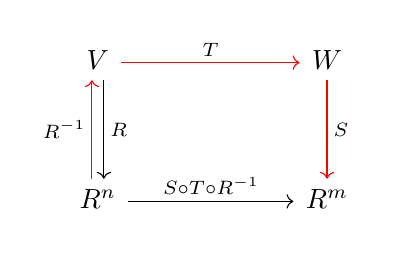
\begin{tikzpicture}
\node{
\begin{tikzcd}[column sep=6em, row sep=huge]
V  \arrow[d, "R" black, shift left=0.5ex] \arrow[red]{r}[black]{T}
& W \arrow[red]{d}[black]{S} \\
\RR^n \arrow[u,red, "R^{-1}" black, shift left=0.5ex]\arrow{r}{S\circ T\circ R^{-1}}
& \RR^m
\end{tikzcd}
};
\end{tikzpicture}
\end{center}

This transformation maps the coordinate vectors of vectors in $V$ to the coordinate vectors of their images in $W$.  For example, if $\vec{v}\mapsto\vec{w}$, then $S\circ T\circ R^{-1}$ accomplishes the following:
$$[\vec{v}]_{\mathcal{B}}\mapsto\vec{v}=a_1\vec{v}_1+a_2\vec{v}_2+\ldots +a_n\vec{v}_n\mapsto\vec{w}=b_1\vec{w}_1+b_2\vec{w}_2+\ldots +b_m\vec{w}_m\mapsto[\vec{w}]_{\mathcal{C}}$$
(In our earlier examples we referred to this transformation as the ``mapping of coordinate vectors".)

The linear transformation $S\circ T\circ R^{-1}:\RR^n\rightarrow \RR^m$ has a standard matrix.  To find it, we need to determine the images of standard unit vectors $\vec{e}_i$ under $S\circ T\circ R^{-1}$. We have the following
$$\vec{e}_i=[\vec{v}_i]_{\mathcal{B}}\mapsto \vec{v}_i \mapsto T(\vec{v}_i)\mapsto [T(\vec{v}_i)]_{\mathcal{C}}$$

We summarize this discussion in as a theorem.

\begin{theorem}\label{th:matlintransgeneral}
Let $V$ and $W$ be finite-dimensional vector spaces with bases $\mathcal{B}=\{\vec{v}_1,\vec{v}_2,\ldots,\vec{v}_n\}$ and $\mathcal{C}$, respectively.  Suppose $T:V\rightarrow W$ is a linear transformation.  
$$\text{Let}\quad A=\begin{bmatrix}
           | & |& &|\\
		[T(\vec{v}_1)]_{\mathcal{C}} & [T(\vec{v}_2)]_{\mathcal{C}}&\dots &[T(\vec{v}_n)]_{\mathcal{C}}\\
		|&| & &|
         \end{bmatrix}$$
Then $A[\vec{v}]_{\mathcal{B}}=[T(\vec{v})]_{\mathcal{C}}$ for all vectors $\vec{v}$ in $V$.       
\end{theorem}

\begin{definition}\label{def:matlintransgenera}
Matrix $A$ of Theorem \ref{th:matlintransgeneral} is called the matrix of $T$ with respect to $\mathcal{B}$ and $\mathcal{C}$.
\end{definition}

In conclusion, observe how isomorphisms helped us solve the matrix of a linear transformation problem.  The coordinate mappings $R$ and $S$ are isomorphisms.  This means that $V$ and $\RR^n$ are isomorphic and have the same structural properties.  The same is true for $W$ and $\RR^m$.  In this abstract discussion, we do not know anything about the elements of $V$ and $W$, but isomorphisms allow us to take a problem that we do not know much about and transform it to a familiar problem involving familiar spaces.

\section*{The Inverse of a Linear Transformation and its Matrix}

Let $V$ and $W$ be vector spaces with bases $\mathcal{B}=\{\vec{v}_1, \vec{v}_2,\ldots ,\vec{v}_n\}$ and $\mathcal{C}=\{\vec{w}_1, \vec{w}_2,\ldots ,\vec{w}_m\}$, respectively.   Suppose $T:V\rightarrow W$ is an invertible linear transformation.  We can find the matrix of $T^{-1}$ with respect to $\mathcal{C}$ and $\mathcal{B}$ by finding the standard matrix of the linear transformation $R\circ T^{-1}\circ S^{-1}:\RR^m\rightarrow \RR^n$.

\begin{center}
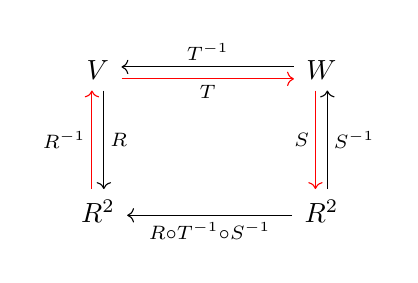
\begin{tikzpicture}
\node{
\begin{tikzcd}[column sep=6em, row sep=huge]
V  \arrow[d, "R" black, shift left=0.5ex] \arrow[r,red, "T"' black, shift right=0.5ex]
& W \arrow[d,red, "S"' black, shift right=0.5ex]\arrow[l, "T^{-1}"' black, shift right=0.5ex] \\
\RR^2 \arrow[u,red, "R^{-1}" black, shift left=0.5ex]
& \RR^2\arrow[u, "S^{-1}"' black, shift right=0.5ex]\arrow{l}{R\circ T^{-1}\circ S^{-1}}
\end{tikzcd}
};
\end{tikzpicture}
\end{center}

Suppose $A$ of  is  the matrix of $T$ with respect to $\mathcal{B}$ and $\mathcal{C}$.  We leave it as an exercise to show that $A^{-1}$ is the matrix of $T^{-1}$ with respect to $\mathcal{C}$ and $\mathcal{B}$.

\begin{example}\label{ex:inversematrixoftransform}
In Exploration Problem \ref{init:subtosub} of LTR-M-0030, we introduced the following set up.

Let $$V=\text{span}\left(\begin{bmatrix}1\\0\\0\end{bmatrix}, \begin{bmatrix}1\\1\\1\end{bmatrix}\right)$$
Define a linear transformation $$T:V\rightarrow \RR^2$$
by $$T\left(\begin{bmatrix}1\\0\\0\end{bmatrix}\right)=\begin{bmatrix}1\\1\end{bmatrix}\quad \text{and} \quad T\left(\begin{bmatrix}1\\1\\1\end{bmatrix}\right)=\begin{bmatrix}0\\1\end{bmatrix}$$

In Example \ref{ex:subtosubinvert} of LTR-M-0035, we proved that $T$ is invertible.  Find the matrix of $T^{-1}$ with respect to bases $\mathcal{C}=\left\{\begin{bmatrix}1\\0\end{bmatrix},\begin{bmatrix}0\\1\end{bmatrix}\right\}$ and $\mathcal{B}=\left\{\begin{bmatrix}1\\0\\0\end{bmatrix}, \begin{bmatrix}1\\1\\1\end{bmatrix}\right\}$
\begin{explanation}
Observe that 
$$T\left(\begin{bmatrix}1\\0\\0\end{bmatrix}\right)=\begin{bmatrix}1\\1\end{bmatrix}=\begin{bmatrix}1\\0\end{bmatrix}+\begin{bmatrix}0\\1\end{bmatrix}\quad \text{and} \quad T\left(\begin{bmatrix}1\\1\\1\end{bmatrix}\right)=\begin{bmatrix}0\\1\end{bmatrix}$$
This gives us the matrix of $T$ with respect to $\mathcal{B}$ and $\mathcal{C}$:
$$A=\begin{bmatrix}\answer{1}&\answer{0}\\\answer{1}&\answer{1}\end{bmatrix}$$
We now find $A^{-1}$. 
$$A^{-1}=\begin{bmatrix}\answer{1}&\answer{0}\\\answer{-1}&\answer{1}\end{bmatrix}$$
$A^{-1}$ is the matrix of $T^{-1}$ with respect to $\mathcal{C}$ and $\mathcal{B}$.
\end{explanation}

\end{example}

\section*{Practice Problems}
\begin{problem}
In Example \ref{ex:transmatrix2} we found the matrix of a linear transformation $T$ with respect to bases $\mathcal{B}$ and $\mathcal{C}$.  Find the matrix of $T$ with respect to the standard bases and compare the two matrices.
\end{problem}

\begin{problem}
Let $V$ and $W$ be vector spaces with bases $\mathcal{B}=\{\vec{v}_1, \vec{v}_2\}$ and $\mathcal{C}=\{\vec{w}_1, \vec{w}_2, \vec{w}_3\}$, respectively.  Define a linear transformation $T:V\rightarrow W$ by $$T(\vec{v}_1)=\vec{w}_1+2\vec{w}_2-\vec{w}_3,\quad T(\vec{v}_2)=3\vec{w}_2+\vec{w}_3$$
Find the matrix $A$ of $T$ with respect to $\mathcal{B}$ and $\mathcal{C}$, and use it to find $T(-\vec{v}_1-3\vec{v}_2)$.  Verify your answer by computing $T(-\vec{v}_1-3\vec{v}_2)$ directly.

$$A=\begin{bmatrix}\answer{1}&\answer{0}\\\answer{2}&\answer{3}\\\answer{-1}&\answer{1}\end{bmatrix}$$

$$T(-\vec{v}_1-3\vec{v}_2)=\answer{-1}\vec{w}_1+\answer{-11}\vec{w}_2+\answer{-2}\vec{w}_3$$
\end{problem}

\begin{problem}
Let $$\vec{v}_1=\begin{bmatrix}2\\0\\1\end{bmatrix}\quad\text{and}\quad\vec{v}_2=\begin{bmatrix}3\\1\\1\end{bmatrix}$$
$$\vec{w}_1=\begin{bmatrix}-1\\1\\1\end{bmatrix}\quad\text{and}\quad\vec{w}_2=\begin{bmatrix}1\\1\\0\end{bmatrix}$$
Let $V$ and $W$ be subspaces of $\RR^3$ with bases $$\mathcal{B}=\{\vec{v}_1, \vec{v}_2\}\quad\text{and}\quad\mathcal{C}=\{\vec{w}_1, \vec{w}_2\}$$
respectively.

Let $T:V\rightarrow W$ be a linear transformation such that 
$$T(\vec{v}_1)=\begin{bmatrix}-1\\3\\2\end{bmatrix}\quad\text{and}\quad T(\vec{v}_2)=\begin{bmatrix}2\\4\\1\end{bmatrix}$$

	\begin{problem}
    Show that $\begin{bmatrix}-1\\3\\2\end{bmatrix}, \begin{bmatrix}2\\4\\1\end{bmatrix}$ lie in $W$ by expressing them as linear combinations of $\vec{w}_1$ and $\vec{w}_2$.
     $$\begin{bmatrix}-1\\3\\2\end{bmatrix}=\answer{2}\vec{w}_1+\answer{1}\vec{w}_2$$
    $$\begin{bmatrix}2\\4\\1\end{bmatrix}=\answer{1}\vec{w}_1+\answer{3}\vec{w}_2$$
    \end{problem}

	\begin{problem}
    Find the matrix of $T$ with respect to $\mathcal{B}$ and $\mathcal{C}$.
    
    $$\begin{bmatrix}\answer{2}&\answer{1}\\\answer{1}&\answer{3}\end{bmatrix}$$
    \end{problem}

	\begin{problem}
    Find the matrix of $T^{-1}$ with respect to $\mathcal{C}$ and $\mathcal{B}$.
    
    $$\begin{bmatrix}\answer{3/5}&\answer{-1/5}\\\answer{-1/5}&\answer{2/5}\end{bmatrix}$$
    \end{problem}
    
    \begin{problem}
    Find $T^{-1}\left(\begin{bmatrix}10\\10\\0\end{bmatrix}\right)$.
    
    $$T^{-1}\left(\begin{bmatrix}10\\10\\0\end{bmatrix}\right)=\begin{bmatrix}\answer{8}\\\answer{4}\\\answer{2}\end{bmatrix}$$
    \end{problem}

\end{problem}

\begin{problem}\label{prob:coordinatemappingisanisom}
In the discussion preceding Theorem \ref{th:matlintransgeneral}, we claimed that $R:V\rightarrow \RR^n$ is an isomorphism.  Prove this by showing that $R$ is one-to-one and onto.  (This problem is the same as Practice Problem \ref{prob:verifyisomorphism}.)
\end{problem}

\begin{problem} Suppose that $T:V\rightarrow W$ is an invertible linear transformation.  Let $A$ be the matrix of $T$ with respect to bases $\mathcal{B}$ and $\mathcal{C}$.  Prove that $A^{-1}$ is the matrix of $T^{-1}$ with respect to bases $\mathcal{C}$ and $\mathcal{B}$.
\end{problem}


%%%%%%Complete diagrams%%%%%%%



%\begin{tikzcd}[column sep=6em, row sep=huge]
%V  \arrow{d}{R} \arrow[red]{r}[black]{T}
%& W \arrow[red]{d}[black]{S} \\
%\RR^2 \arrow[u,red, "R^{-1}" black, shift left=1.5ex]\arrow{r}{S\circ T\circ R^{-1}}
%& \RR^2
%\end{tikzcd}

%  \begin{tikzcd}[column sep=6em, row sep=huge]
%\vec{v}=a\vec{v}_1+b\vec{v}_2  \arrow[d,mapsto]\arrow[r,red,mapsto]
%& (2a-b)\vec{w}_1+(3a+2b)\vec{w}_2 \arrow[d, red, mapsto] \\
%\begin{bmatrix}a\\b\end{bmatrix} \arrow[u,red, mapsto, shift left=1.5ex]\arrow[r, mapsto]
%& \begin{bmatrix}2a-b\\3a+2b\end{bmatrix}
%\end{tikzcd}

 % \begin{tikzcd}[column sep=6em, row sep=huge]
%\vec{v}_1 \arrow[d,mapsto]\arrow[r,red,mapsto]
%& T(\vec{v}_1)=2\vec{w}_1+3\vec{w}_2 \arrow[d, red, mapsto] \\
%\begin{bmatrix}1\\0\end{bmatrix} \arrow[u,red, mapsto, shift left=1.5ex]\arrow[r, mapsto]
%& \begin{bmatrix}2\\3\end{bmatrix}
%\end{tikzcd}\quad
%\begin{tikzcd}[column sep=6em, row sep=huge]
%\vec{v}_2 \arrow[d,mapsto]\arrow[r,red,mapsto]
%& T(\vec{v}_2)=-\vec{w}_1+2\vec{w}_2 \arrow[d, red, mapsto] \\
%\begin{bmatrix}0\\1\end{bmatrix} \arrow[u,red, mapsto, shift left=1.5ex]\arrow[r, mapsto]
%& \begin{bmatrix}-1\\2\end{bmatrix}
%\end{tikzcd}

 

\end{document}
